\documentclass{beamer}
\usepackage{beamerthemeshadow}
\usepackage{color}
%\usepackage[all]{xy}


%%%% choose your presentation style:
\mode<presentation>
{
  \usetheme{Copenhagen} %%%
 \usecolortheme{beaver}

%%% set style for ovelays: lists (and other text) appearing one item at a time
%%% This will create a dimmed preview of next item:
\setbeamercovered{transparent}
%%% This will hide it entirely:
%\setbeamercovered{invisible}
}
%% if you don't want page numbers to show: 
\setbeamertemplate{footline}[page number]{}
\usenavigationsymbolstemplate{}


\begin{document}
\title{Parallel BVH Construction for Real-Time Ray Tracing}
\author{Aaron Lemmon}
\institute[UMM] % (optional, but mostly needed)
{
 % \inst{1}%
  University of Minnesota, Morris
}
\date[]  
{April 30, 2015}

\begin{frame}
  \titlepage
\end{frame}

\begin{frame}
  \frametitle{Ray Traced Scene}
\begin{figure}
%%% note: the file is in the same folder as your .tex file
\includegraphics[height=60mm]{Glasses_800_edit.png}
\urlstyle{rm}
\hspace{6pt}\hbox{\tiny{\url{https://en.wikipedia.org/wiki/Ray_tracing_(graphics)}}}
\end{figure}

%\hspace{12pt}\hbox{\scriptsize Credit:\thinspace{\small\itshape Kathleen Gilje}}


%\href{https://en.wikipedia.org/wiki/Ray_tracing_(graphics)}{https://en.wikipedia.org/wiki/Ray_tracing_(graphics)}
\end{frame}

\begin{frame}

  \frametitle{Outline}
\tableofcontents
\end{frame}

\section{Ray Tracing Fundamentals}

\begin{frame}
  \frametitle{Primitives}
\begin{figure}
%%% note: the file is in the same folder as your .tex file
\includegraphics[height=60mm]{Dolphin_triangle_mesh.png}
\urlstyle{rm}
\hspace{6pt}\hbox{\tiny{\url{https://en.wikipedia.org/wiki/Triangle_mesh}}}
\end{figure}
\end{frame}

\begin{frame}
  \frametitle{Ray Tracing}
\begin{figure}
%%% note: the file is in the same folder as your .tex file
\includegraphics[height=60mm]{Ray_trace_diagram.pdf}
\urlstyle{rm}
\hspace{6pt}\hbox{\tiny{\url{https://en.wikipedia.org/wiki/Ray_tracing_(graphics)}}}
\end{figure}
\end{frame}

\begin{frame}
  \frametitle{Axis-Aligned Bounding Boxes}
\begin{figure}
%%% note: the file is in the same folder as your .tex file
\includegraphics[height=60mm]{aabb.png}
\urlstyle{rm}
\hspace{6pt}\hbox{\tiny{\url{http://www.scratchapixel.com}}}
\end{figure}
\end{frame}

\section{Grouping Primitives}

\begin{frame}
  \frametitle{Bounding Volume Hierarchy}
  
\begin{columns}[t]

\column{.5\textwidth}
\begin{figure}
%%% note: the file is in the same folder as your .tex file
\includegraphics[height=45mm]{build0.png}
\end{figure}

\column{.5\textwidth}
\begin{figure}
%%% note: the file is in the same folder as your .tex file
\includegraphics[height=45mm]{primitive_tree_narrow.png}
\end{figure}
\end{columns}
\end{frame}

\begin{frame}
  \frametitle{Bounding Volume Hierarchy}
  
\begin{columns}[t]

\column{.5\textwidth}
\begin{figure}
%%% note: the file is in the same folder as your .tex file
\includegraphics[height=45mm]{build1.png}
\end{figure}

\column{.5\textwidth}
\begin{figure}
%%% note: the file is in the same folder as your .tex file
\includegraphics[height=45mm]{primitive_tree_narrow.png}
\end{figure}
\end{columns}
\end{frame}

\begin{frame}
  \frametitle{Bounding Volume Hierarchy}
  
\begin{columns}[t]

\column{.5\textwidth}
\begin{figure}
%%% note: the file is in the same folder as your .tex file
\includegraphics[height=45mm]{build2.png}
\end{figure}

\column{.5\textwidth}
\begin{figure}
%%% note: the file is in the same folder as your .tex file
\includegraphics[height=45mm]{primitive_tree_narrow.png}
\end{figure}
\end{columns}
\end{frame}

\begin{frame}
  \frametitle{Bounding Volume Hierarchy}
  
\begin{columns}[t]

\column{.5\textwidth}
\begin{figure}
%%% note: the file is in the same folder as your .tex file
\includegraphics[height=45mm]{build3.png}
\end{figure}

\column{.5\textwidth}
\begin{figure}
%%% note: the file is in the same folder as your .tex file
\includegraphics[height=45mm]{primitive_tree_narrow.png}
\end{figure}
\end{columns}
\end{frame}

\begin{frame}
  \frametitle{Bounding Volume Hierarchy}
  
\begin{columns}[t]

\column{.5\textwidth}
\begin{figure}
%%% note: the file is in the same folder as your .tex file
\includegraphics[height=45mm]{build4.png}
\end{figure}

\column{.5\textwidth}
\begin{figure}
%%% note: the file is in the same folder as your .tex file
\includegraphics[height=45mm]{primitive_tree_narrow.png}
\end{figure}
\end{columns}
\end{frame}

\begin{frame}
  \frametitle{Bounding Volume Hierarchy}
  
\begin{columns}[t]

\column{.5\textwidth}
\begin{figure}
%%% note: the file is in the same folder as your .tex file
\includegraphics[height=45mm]{primitive-box-ray.png}
\end{figure}

\column{.5\textwidth}
\begin{figure}
%%% note: the file is in the same folder as your .tex file
\includegraphics[height=45mm]{primitive_tree_narrow.png}
\end{figure}
\end{columns}
\end{frame}

\begin{frame}
  \frametitle{Bounding Volume Hierarchy}
  
\begin{columns}[t]

\column{.5\textwidth}
\begin{figure}
%%% note: the file is in the same folder as your .tex file
\includegraphics[height=45mm]{primitive-box-ray.png}
\end{figure}

\column{.5\textwidth}
\begin{figure}
%%% note: the file is in the same folder as your .tex file
\includegraphics[height=45mm]{elim_0.png}
\end{figure}
\end{columns}
\end{frame}

\begin{frame}
  \frametitle{Bounding Volume Hierarchy}
  
\begin{columns}[t]

\column{.5\textwidth}
\begin{figure}
%%% note: the file is in the same folder as your .tex file
\includegraphics[height=45mm]{primitive-box-ray.png}
\end{figure}

\column{.5\textwidth}
\begin{figure}
%%% note: the file is in the same folder as your .tex file
\includegraphics[height=45mm]{elim_1.png}
\end{figure}
\end{columns}
\end{frame}

\begin{frame}
  \frametitle{Bounding Volume Hierarchy}
  
\begin{columns}[t]

\column{.5\textwidth}
\begin{figure}
%%% note: the file is in the same folder as your .tex file
\includegraphics[height=45mm]{primitive-box-ray.png}
\end{figure}

\column{.5\textwidth}
\begin{figure}
%%% note: the file is in the same folder as your .tex file
\includegraphics[height=45mm]{elim_2.png}
\end{figure}
\end{columns}
\end{frame}

%\begin{frame}
%  \frametitle{Scene}
%\begin{figure}
%%%% note: the file is in the same folder as your .tex file
%\includegraphics[height=45mm]{Z-curve-primitives.png}
%\end{figure}
%\end{frame}

\begin{frame}
  \frametitle{Morton Codes}
  
\begin{columns}[t]

\column{.5\textwidth}
\begin{figure}
%%% note: the file is in the same folder as your .tex file
\includegraphics[height=55mm]{Z-curve-primitives.png}
\end{figure}

\column{.5\textwidth}
\begin{figure}
%%% note: the file is in the same folder as your .tex file
\includegraphics[height=55mm]{Z-curve-zoomed.png}
\end{figure}
\end{columns}
\end{frame}

\begin{frame}
  \frametitle{Morton Codes}
\begin{figure}
%%% note: the file is in the same folder as your .tex file
\includegraphics[height=70mm]{Z-curve.png}
\end{figure}
\end{frame}

%\begin{frame}
%  \frametitle{Morton Codes}
%\begin{columns}[t]
%
%\column{.5\textwidth}
%\centering
%\begin{itemize}
%\item Interleave binary representations of coordinate values
%\item Transforms multidimensional coordinates into a single value
%\item Morton Code contains location information
%\item Used to sort objects
%\end{itemize}
%
%\column{.5\textwidth}
%\begin{figure}
%%%% note: the file is in the same folder as your .tex file
%\includegraphics[height=45mm]{Z-curve.pdf}
%\end{figure}
%\end{columns}
%\end{frame}

%\begin{frame}
%  \frametitle{Shape of a Z-order Curve}
%\begin{figure}
%%%% note: the file is in the same folder as your .tex file
%\includegraphics[height=45mm]{542px-Four-level_Z.png}
%\end{figure}
%\end{frame}

\begin{frame}
  \frametitle{Morton Codes}
\begin{figure}
%%% note: the file is in the same folder as your .tex file
\includegraphics[height=70mm]{Z-curve-primitives.png}
\end{figure}
\end{frame}

\begin{frame}
  \frametitle{Morton Codes}
  
\begin{columns}[t]

\column{.5\textwidth}
\begin{figure}
%%% note: the file is in the same folder as your .tex file
\includegraphics[height=55mm]{Z-curve-primitives.png}
\end{figure}

\column{.5\textwidth}
\begin{figure}
%%% note: the file is in the same folder as your .tex file
%\includegraphics[height=55mm]{keys_0.png}
\end{figure}
\end{columns}
\end{frame}

\begin{frame}
  \frametitle{Morton Codes}
  
\begin{columns}[t]

\column{.5\textwidth}
\begin{figure}
%%% note: the file is in the same folder as your .tex file
\includegraphics[height=55mm]{Z-curve-primitives.png}
\end{figure}

\column{.5\textwidth}
\begin{figure}
%%% note: the file is in the same folder as your .tex file
\includegraphics[height=55mm]{keys_0.png}
\end{figure}
\end{columns}
\end{frame}

\begin{frame}
  \frametitle{Morton Codes}
  
\begin{columns}[t]

\column{.5\textwidth}
\begin{figure}
%%% note: the file is in the same folder as your .tex file
\includegraphics[height=55mm]{Z-curve-primitives.png}
\end{figure}

\column{.5\textwidth}
\begin{figure}
%%% note: the file is in the same folder as your .tex file
\includegraphics[height=55mm]{keys_1.png}
\end{figure}
\end{columns}
\end{frame}

\begin{frame}
  \frametitle{Morton Codes}
  
\begin{columns}[t]

\column{.5\textwidth}
\begin{figure}
%%% note: the file is in the same folder as your .tex file
\includegraphics[height=55mm]{Z-curve-primitives.png}
\end{figure}

\column{.5\textwidth}
\begin{figure}
%%% note: the file is in the same folder as your .tex file
\includegraphics[height=55mm]{keys_2.png}
\end{figure}
\end{columns}
\end{frame}

\begin{frame}
  \frametitle{Morton Codes}
  
\begin{columns}[t]

\column{.5\textwidth}
\begin{figure}
%%% note: the file is in the same folder as your .tex file
\includegraphics[height=55mm]{Z-curve-primitives.png}
\end{figure}

\column{.5\textwidth}
\begin{figure}
%%% note: the file is in the same folder as your .tex file
\includegraphics[height=55mm]{keys_3.png}
\end{figure}
\end{columns}
\end{frame}

\begin{frame}
  \frametitle{Morton Codes}
  
\begin{columns}[t]

\column{.5\textwidth}
\begin{figure}
%%% note: the file is in the same folder as your .tex file
\includegraphics[height=55mm]{Z-curve-primitives.png}
\end{figure}

\column{.5\textwidth}
\begin{figure}
%%% note: the file is in the same folder as your .tex file
\includegraphics[height=55mm]{keys_4.png}
\end{figure}
\end{columns}
\end{frame}

\begin{frame}
  \frametitle{Morton Codes}
  
\begin{columns}[t]

\column{.5\textwidth}
\begin{figure}
%%% note: the file is in the same folder as your .tex file
\includegraphics[height=55mm]{Z-curve-primitives.png}
\end{figure}

\column{.5\textwidth}
\begin{figure}
%%% note: the file is in the same folder as your .tex file
\includegraphics[height=55mm]{keys_5.png}
\end{figure}
\end{columns}
\end{frame}

\begin{frame}
  \frametitle{Morton Codes}
  
\begin{columns}[t]

\column{.5\textwidth}
\begin{figure}
%%% note: the file is in the same folder as your .tex file
\includegraphics[height=55mm]{Z-curve-primitives.png}
\end{figure}

\column{.5\textwidth}
\begin{figure}
%%% note: the file is in the same folder as your .tex file
\includegraphics[height=55mm]{keys_6.png}
\end{figure}
\end{columns}
\end{frame}

\begin{frame}
  \frametitle{Morton Codes}
  
\begin{columns}[t]

\column{.5\textwidth}
\begin{figure}
%%% note: the file is in the same folder as your .tex file
\includegraphics[height=55mm]{Z-curve-primitives.png}
\end{figure}

\column{.5\textwidth}
\begin{figure}
%%% note: the file is in the same folder as your .tex file
\includegraphics[height=55mm]{keys_7.png}
\end{figure}
\end{columns}
\end{frame}

\section{Bounding Volume Hierarchy Construction}

\begin{frame}
  \frametitle{Goal}
  
\begin{columns}[t]

\column{.5\textwidth}
\begin{figure}
%%% note: the file is in the same folder as your .tex file
\includegraphics[height=45mm]{primitive-box.png}
\end{figure}

\column{.5\textwidth}
\begin{figure}
%%% note: the file is in the same folder as your .tex file
\includegraphics[height=55mm]{radix_tree_bare.png}
\end{figure}
\end{columns}
\end{frame}

\begin{frame}
  \frametitle{Binary Radix Tree}
  
\begin{columns}[t]

\column{.5\textwidth}
\begin{figure}
%%% note: the file is in the same folder as your .tex file
\includegraphics[height=45mm]{primitive-box.png}
\end{figure}

\column{.5\textwidth}
\begin{figure}
%%% note: the file is in the same folder as your .tex file
\includegraphics[height=55mm]{full_radix_tree_narrow.png}
\end{figure}
\end{columns}
\end{frame}

\begin{frame}
  \frametitle{Internal Node Array}
  
\begin{columns}[t]

\column{.5\textwidth}
\begin{figure}
%%% note: the file is in the same folder as your .tex file
\includegraphics[height=45mm]{primitive-box.png}
\end{figure}

\column{.5\textwidth}
\begin{figure}
%%% note: the file is in the same folder as your .tex file
\includegraphics[height=55mm]{full_tree_arrays_narrow.png}
\end{figure}
\end{columns}
\end{frame}

\begin{frame}
  \frametitle{Internal Nodes}
  
\begin{columns}[t]

\column{.5\textwidth}
\begin{figure}
%%% note: the file is in the same folder as your .tex file
\includegraphics[height=45mm]{primitive-box.png}
\end{figure}

\column{.5\textwidth}
\begin{figure}
%%% note: the file is in the same folder as your .tex file
\includegraphics[height=55mm]{algo_0.png}
\end{figure}
\end{columns}
\end{frame}

\begin{frame}
  \frametitle{Determine Range Direction}
  
\begin{columns}[t]

\column{.5\textwidth}
\begin{figure}
%%% note: the file is in the same folder as your .tex file
\includegraphics[height=45mm]{primitive-box.png}
\end{figure}

\column{.5\textwidth}
\begin{figure}
%%% note: the file is in the same folder as your .tex file
\includegraphics[height=55mm]{algo_1.png}
\end{figure}
\end{columns}
\end{frame}

\begin{frame}
  \frametitle{Determine Full Range}
  
\begin{columns}[t]

\column{.5\textwidth}
\begin{figure}
%%% note: the file is in the same folder as your .tex file
\includegraphics[height=45mm]{primitive-box.png}
\end{figure}

\column{.5\textwidth}
\begin{figure}
%%% note: the file is in the same folder as your .tex file
\includegraphics[height=55mm]{algo_2.png}
\end{figure}
\end{columns}
\end{frame}

\begin{frame}
  \frametitle{Determine Split Location}
  
\begin{columns}[t]

\column{.5\textwidth}
\begin{figure}
%%% note: the file is in the same folder as your .tex file
\includegraphics[height=45mm]{primitive-box.png}
\end{figure}

\column{.5\textwidth}
\begin{figure}
%%% note: the file is in the same folder as your .tex file
\includegraphics[height=55mm]{algo_3.png}
\end{figure}
\end{columns}
\end{frame}

\begin{frame}
  \frametitle{Determine Children}
  
\begin{columns}[t]

\column{.5\textwidth}
\begin{figure}
%%% note: the file is in the same folder as your .tex file
\includegraphics[height=45mm]{primitive-box.png}
\end{figure}

\column{.5\textwidth}
\begin{figure}
%%% note: the file is in the same folder as your .tex file
\includegraphics[height=55mm]{algo_4.png}
\end{figure}
\end{columns}
\end{frame}

\begin{frame}
  \frametitle{Fitting Boxes}
  
\begin{columns}[t]

\column{.5\textwidth}
\begin{figure}
%%% note: the file is in the same folder as your .tex file
\includegraphics[height=45mm]{fit_0.png}
\end{figure}

\column{.5\textwidth}
\begin{figure}
%%% note: the file is in the same folder as your .tex file
\includegraphics[height=55mm]{radix_tree_bare.png}
\end{figure}
\end{columns}
\end{frame}

\begin{frame}
  \frametitle{Fitting Boxes}
  
\begin{columns}[t]

\column{.5\textwidth}
\begin{figure}
%%% note: the file is in the same folder as your .tex file
\includegraphics[height=45mm]{fit_1.png}
\end{figure}

\column{.5\textwidth}
\begin{figure}
%%% note: the file is in the same folder as your .tex file
\includegraphics[height=55mm]{radix_tree_bare.png}
\end{figure}
\end{columns}
\end{frame}

\begin{frame}
  \frametitle{Fitting Boxes}
  
\begin{columns}[t]

\column{.5\textwidth}
\begin{figure}
%%% note: the file is in the same folder as your .tex file
\includegraphics[height=45mm]{fit_2.png}
\end{figure}

\column{.5\textwidth}
\begin{figure}
%%% note: the file is in the same folder as your .tex file
\includegraphics[height=55mm]{radix_tree_bare.png}
\end{figure}
\end{columns}
\end{frame}

\begin{frame}
  \frametitle{Fitting Boxes}
  
\begin{columns}[t]

\column{.5\textwidth}
\begin{figure}
%%% note: the file is in the same folder as your .tex file
\includegraphics[height=45mm]{fit_3.png}
\end{figure}

\column{.5\textwidth}
\begin{figure}
%%% note: the file is in the same folder as your .tex file
\includegraphics[height=55mm]{radix_tree_bare.png}
\end{figure}
\end{columns}
\end{frame}

\begin{frame}
  \frametitle{Fitting Boxes}
  
\begin{columns}[t]

\column{.5\textwidth}
\begin{figure}
%%% note: the file is in the same folder as your .tex file
\includegraphics[height=45mm]{fit_4.png}
\end{figure}

\column{.5\textwidth}
\begin{figure}
%%% note: the file is in the same folder as your .tex file
\includegraphics[height=55mm]{radix_tree_bare.png}
\end{figure}
\end{columns}
\end{frame}


\section{Results}

\begin{frame}
  \frametitle{Results}
\begin{figure}
%%% note: the file is in the same folder as your .tex file
\includegraphics[height=50mm]{new_cores3.png}
\hspace{6pt}\hbox{\tiny{Tero Karras 2012 [3].}}
\end{figure}
\end{frame}

\begin{frame}
  \frametitle{Results}
\begin{figure}
%%% note: the file is in the same folder as your .tex file
\includegraphics[height=50mm]{new_performance.png}
\hspace{6pt}\hbox{\tiny{Tero Karras 2012 [3].}}
\end{figure}
\end{frame}

%\begin{frame}
%  \frametitle{Binary Radix Tree Example}
%  
%\begin{columns}[t]
%
%\column{.5\textwidth}
%\begin{figure}
%%%% note: the file is in the same folder as your .tex file
%\includegraphics[height=40mm]{BinaryRadixTree.pdf}
%\end{figure}
%
%\column{.5\textwidth}
%\begin{figure}
%%%% note: the file is in the same folder as your .tex file
%\includegraphics[height=40mm]{Z-curve.pdf}
%\end{figure}
%\end{columns}
%\end{frame}

\begin{frame}
  \frametitle{Questions?}
\begin{figure}
%%% note: the file is in the same folder as your .tex file
\includegraphics[height=60mm]{lemon.jpg}
\urlstyle{rm}
\hspace{6pt}\hbox{\tiny{\url{digitaltutors.com}}}
\end{figure}
\end{frame}

\begin{frame}
  \frametitle{Bibliography}
\begin{tiny}
\begin{enumerate}
	\item Kirill Garanzha, Jacopo Pantaleoni, and David McAllister. 2011. Simpler and faster HLBVH with work queues. In Proceedings of the ACM SIGGRAPH Symposium on High Performance Graphics (HPG '11), Stephen N. Spencer (Ed.). ACM, New York, NY, USA, 59-64. DOI=http://dx.doi.org.ezproxy.morris.umn.edu/10.1145/2018323.2018333
	\item Christiaan Gribble, Jeremy Fisher, Daniel Eby, Ed Quigley, and Gideon Ludwig. 2012. Ray tracing visualization toolkit. In Proceedings of the ACM SIGGRAPH Symposium on Interactive 3D Graphics and Games (I3D '12), Stephen N. Spencer (Ed.). ACM, New York, NY, USA, 71-78. DOI=http://dx.doi.org.ezproxy.morris.umn.edu/10.1145/2159616.2159628
	\item Tero Karras. 2012. Maximizing parallelism in the construction of BVHs, octrees, and k-d trees. In Proceedings of the Fourth ACM SIGGRAPH / Eurographics conference on High-Performance Graphics (EGGH-HPG'12), Carsten Dachsbacher, Jacob Munkberg, and Jacopo Pantaleoni (Eds.). Eurographics Association, Aire-la-Ville, Switzerland, Switzerland, 33-37. DOI=http://dx.doi.org.ezproxy.morris.umn.edu/10.2312/EGGH/HPG12/033-037
	\item Timo Viitanen, Matias Koskela, Pekka Jääskeläinen, Heikki Kultala, and Jarmo Takala. 2015. MergeTree: a HLBVH constructor for mobile systems. In SIGGRAPH Asia 2015 Technical Briefs (SA '15). ACM, New York, NY, USA, , Article 12 , 4 pages. DOI=http://dx.doi.org.ezproxy.morris.umn.edu/10.1145/2820903.2820916
	\item Ingo Wald. 2007. On fast Construction of SAH-based Bounding Volume Hierarchies. In Proceedings of the 2007 IEEE Symposium on Interactive Ray Tracing (RT '07). IEEE Computer Society, Washington, DC, USA, 33-40. DOI=http://dx.doi.org/10.1109/RT.2007.4342588
	\item Turner Whitted. 1980. An improved illumination model for shaded display. Commun. ACM 23, 6 (June 1980), 343-349. DOI=http://dx.doi.org/10.1145/358876.358882
\end{enumerate}
\end{tiny}
\end{frame}

\end{document}
